% !TeX root = ../main.tex
\chapter{zPSC Chassis Overview}
\label{chap:chassis_overview}

\section{Introduction}

\section{Front Panels (2- and 4-Channel PSCs)}
Both 2- and 4-Channel units share identical front panels:
\begin{figure}[H]
	\centering
	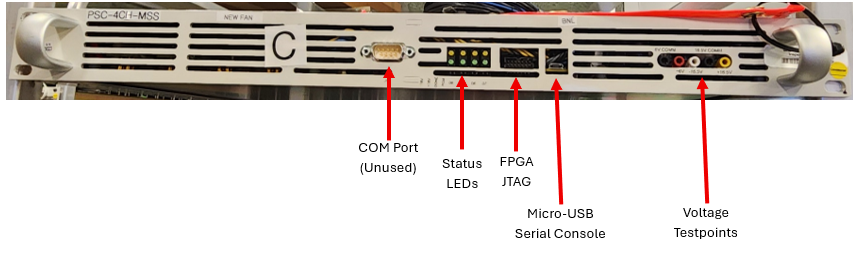
\includegraphics[width=\textwidth]{Pictures/PSC_FP_Annotated}
\end{figure}

\section{Rear Panel - 2 Channel}
\begin{figure}[H]
	\centering
	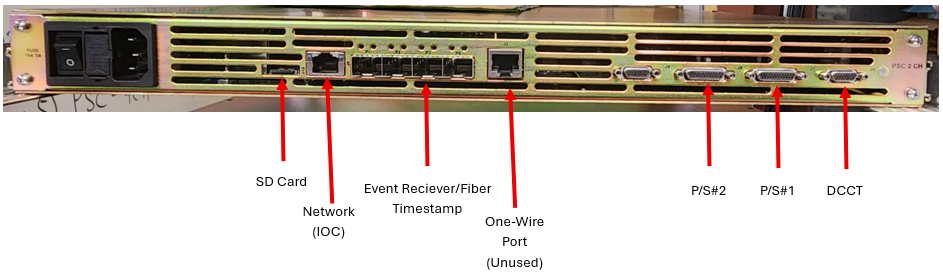
\includegraphics[width=\textwidth]{Pictures/2Ch_PSC_Annotated}
\end{figure}

\section{Internal Component Layout - 2 Channel}
\begin{figure}[H]
	\centering
	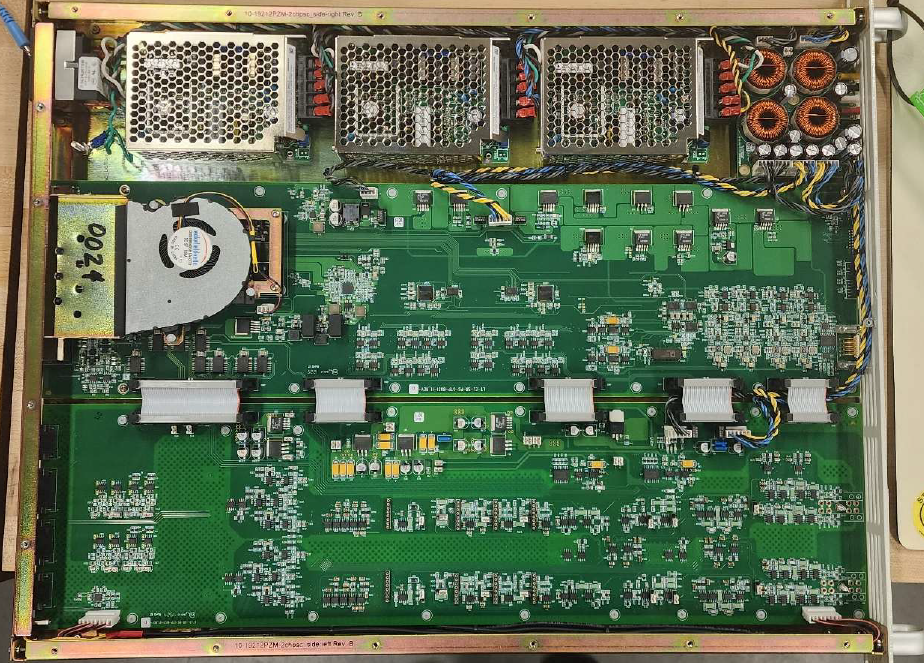
\includegraphics[width=\textwidth]{Pictures/2Ch_PSC_Chassis}
\end{figure}

\subsection{Analog Board Components}
\begin{figure}[H]
	\centering
	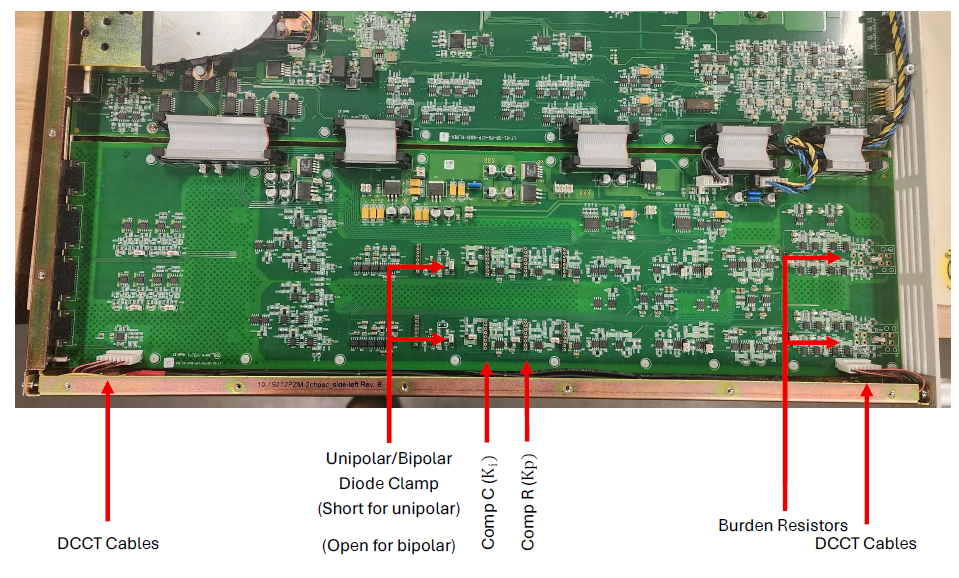
\includegraphics[width=\textwidth]{Pictures/2Ch_PSC_Analog_Brd_Annotated}
\end{figure}

\newpage
\section{Rear Panel - 4 Channel}
\begin{figure}[H]
	\centering
	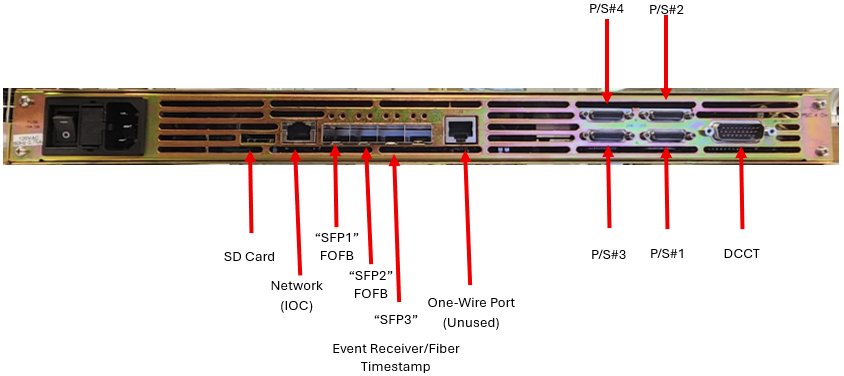
\includegraphics[width=\textwidth]{Pictures/4Ch_PSC_Rear_Annotated}
\end{figure}

\section{Internal Component Layout - 4 Channel}
\begin{figure}[H]
	\centering
	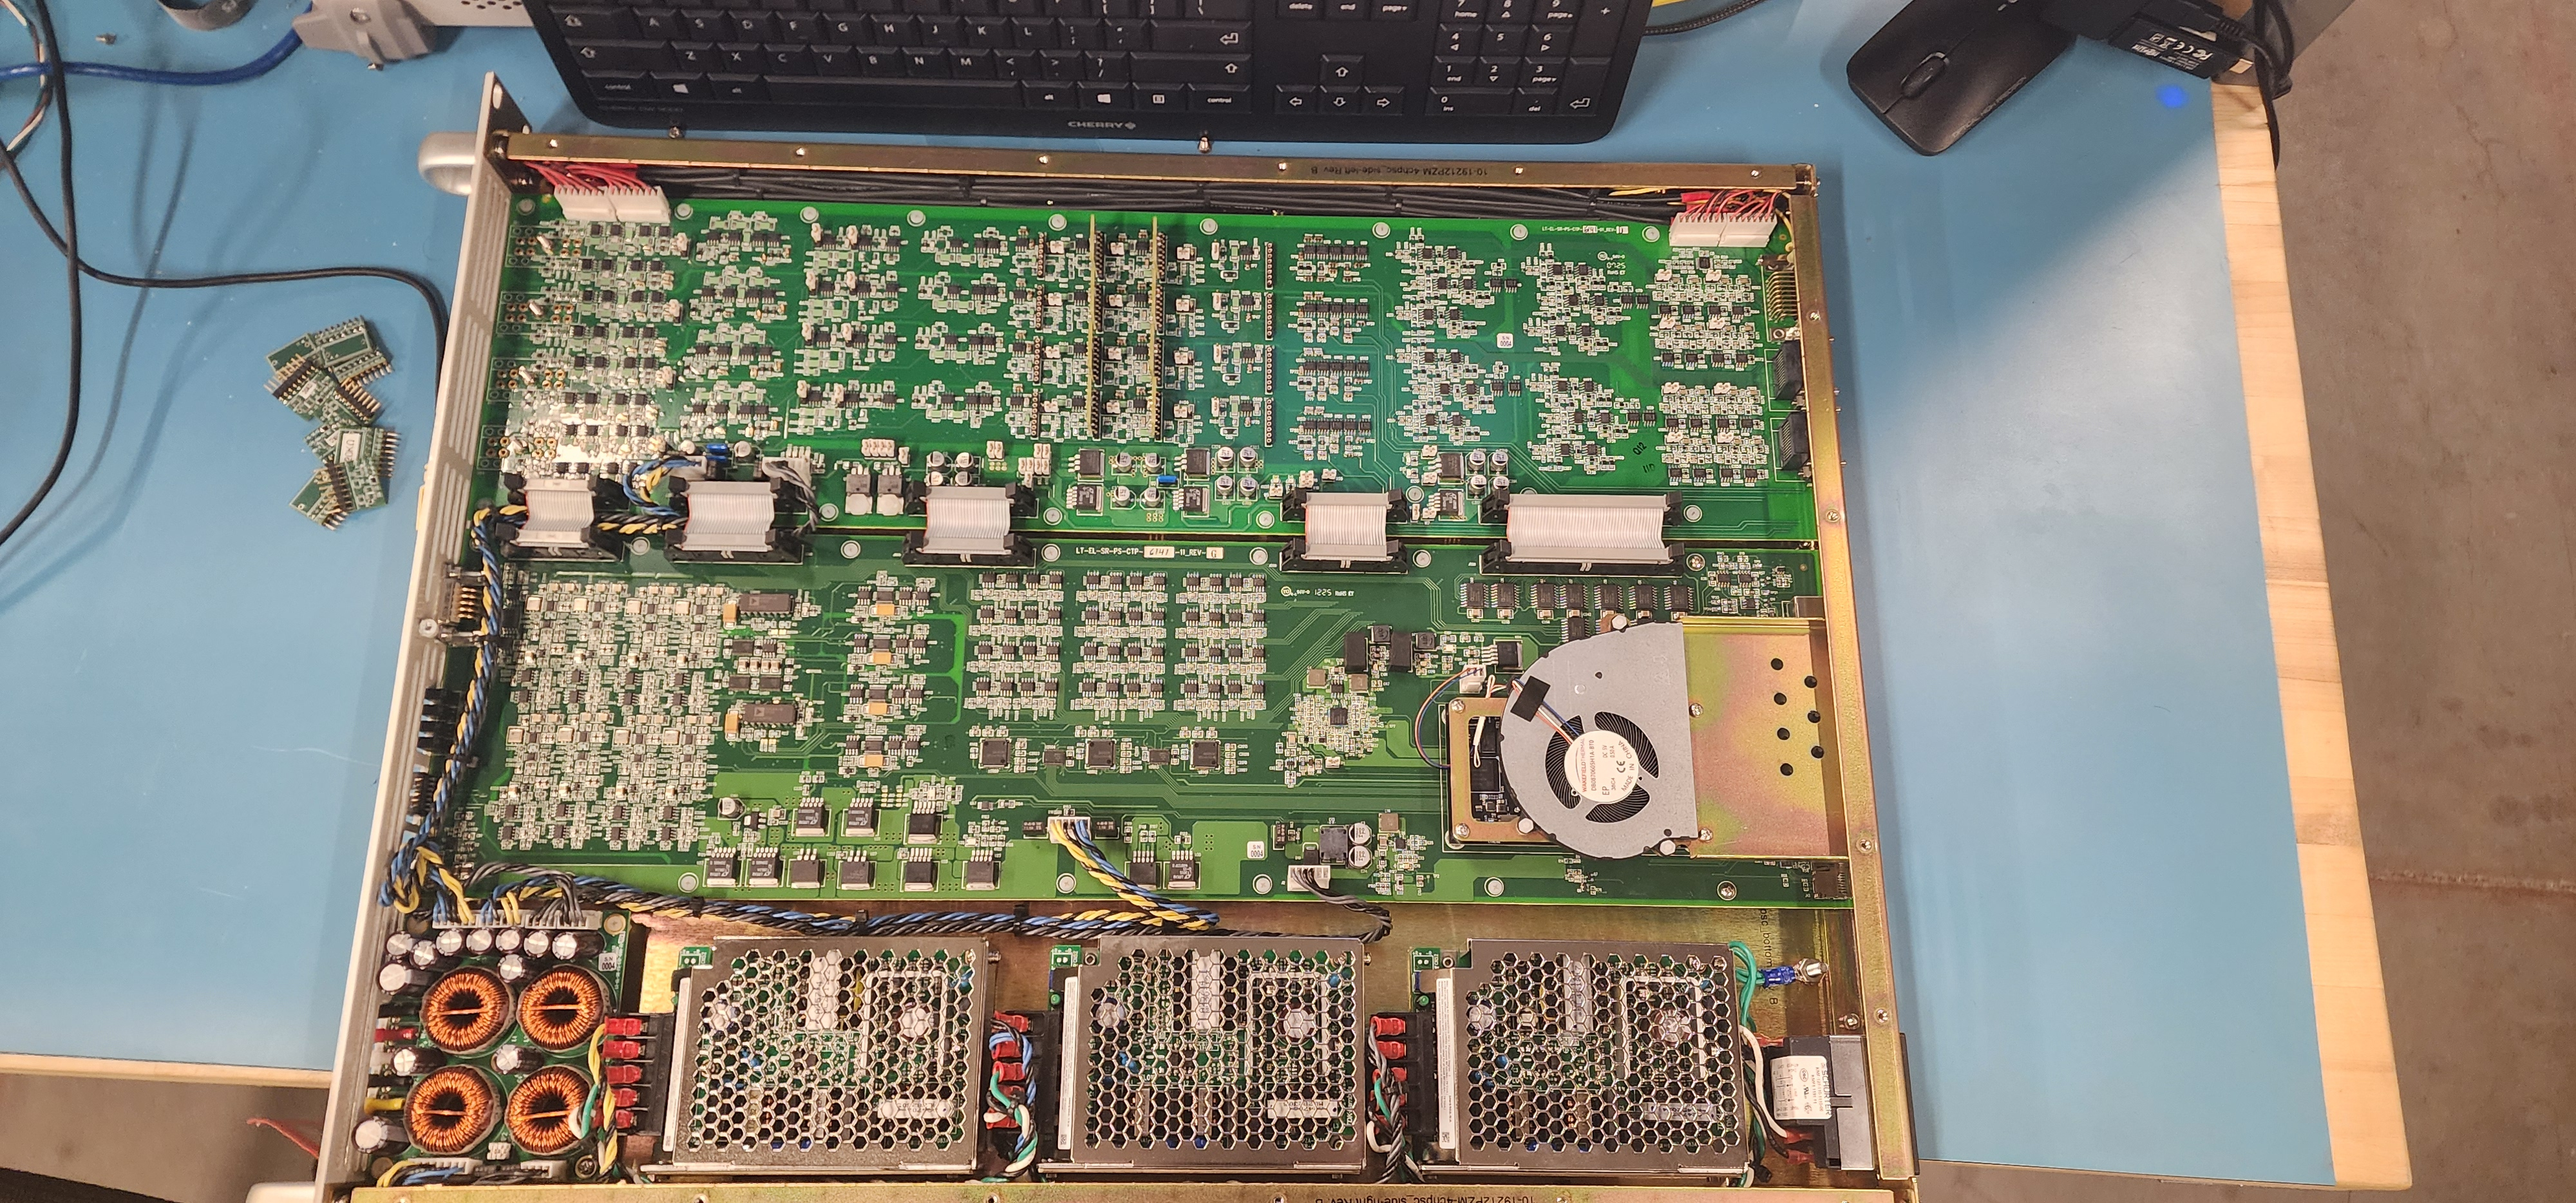
\includegraphics[width=\textwidth]{Pictures/4-Ch_PSC_Top_View}
\end{figure}

\subsection{Analog Board Components}
\begin{figure}[H]
	\centering
	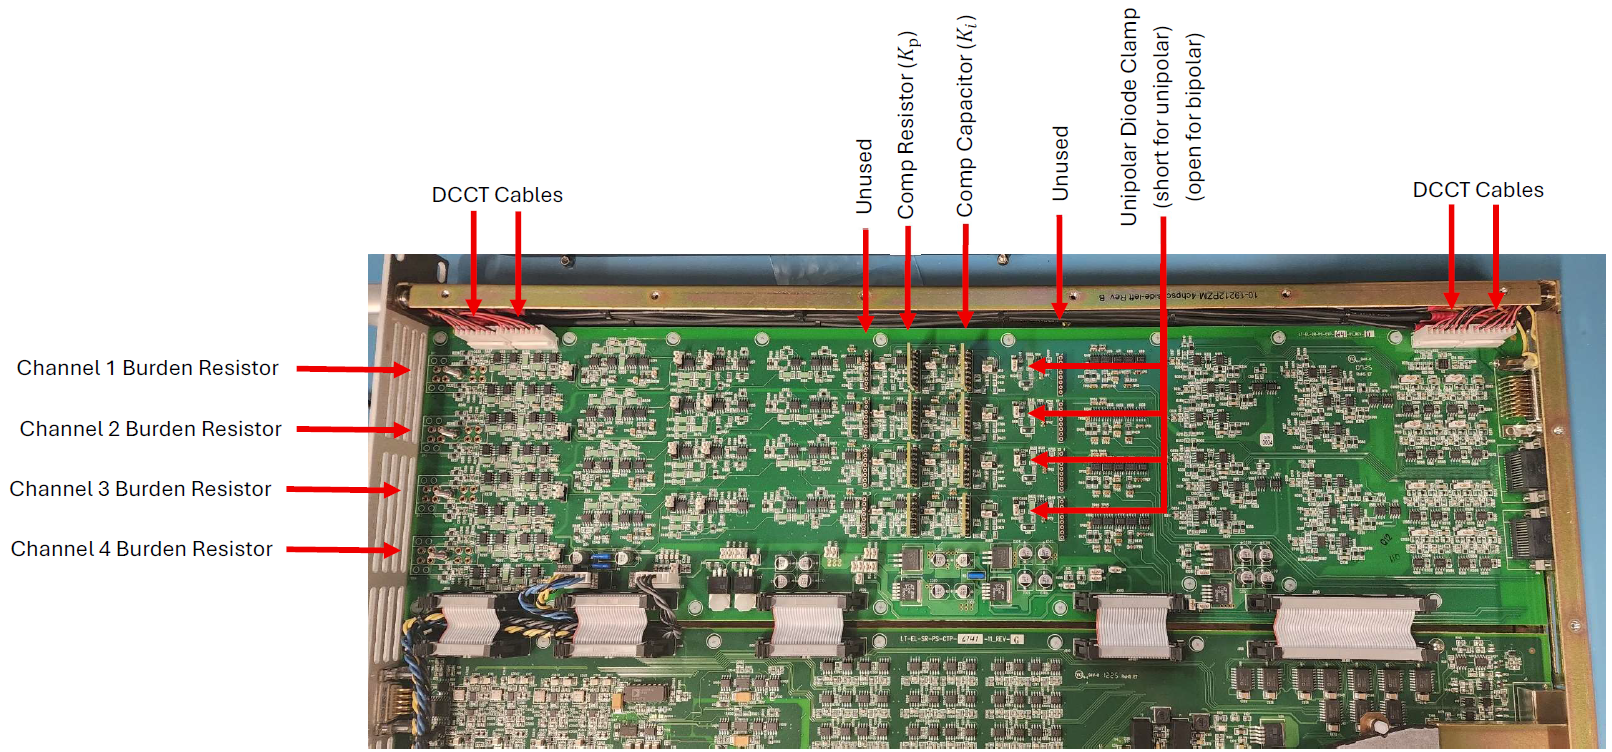
\includegraphics[width=\textwidth]{Pictures/4Ch-PSC_Analog_Brd_Annotated}
\end{figure}

